\documentclass[a4paper]{article}
\usepackage[utf8]{inputenc}
\usepackage[T1]{fontenc}      
\usepackage[english]{babel} %utilisation du package français
%
%
%
\usepackage{textcomp}% améliore certains symboles de bases
\usepackage{lmodern}% remplace la police ComputerModern par LatinModern (+ mieux bien)
%
%
%
\usepackage{mathtools}% compléments à amsmath
\usepackage{amssymb,amsfonts}% symboles mathématiques supplémentaires
\usepackage{amsthm}% environnement ams-theorem
\usepackage[colorlinks,breaklinks,bookmarks,plainpages=false,unicode=true]{hyperref}%
\usepackage{todonotes} %ajouter des commentaires
%\usepackage[disable]{todonotes}%cache les commentaires
\usepackage{datetime} %ajoute la date et l'heure
%
%
\usepackage{tikz}
\usetikzlibrary{external,graphs}
\tikzexternalize[prefix=Images/]% On externalise. Les images sont stockées dans le dossier Images
\makeatletter %pour ne pas prendre en compte les todo dans l'externalisation
\renewcommand{\todo}[2][]{\tikzexternaldisable\@todo[#1]{#2}\tikzexternalenable}
\makeatother
\makeatletter %pour ne pas prendre en compte les missingfigures dans l'externalisation
\renewcommand{\missingfigure}[2][]{\tikzexternaldisable\@missingfigure[#1]{#2}\tikzexternalenable}
\makeatother

\tikzset{myloop above/.style={loop, out=130, in = 50,min distance =8mm}}
\tikzset{myloop below/.style={loop, out=-130, in = -50,min distance =8mm}}
\tikzset{blacknode/.style={shape= circle, fill = black, inner sep = 0pt, outer sep = 0pt, minimum size = 3pt,draw}}
%
\newtheorem{lem}{Lemma}[section]
\newtheorem{conjecture}[lem]{Conjecture}
\newtheorem{cor}[lem]{Corollary}
\newtheorem{prop}[lem]{Proposition}
\newtheorem{thm}[lem]{Theorem}
\theoremstyle{definition}
\newtheorem{defn}[lem]{Definition}
\theoremstyle{remark}% texte en roman
\newtheorem{exmp}[lem]{Example}
%
%
%
\DeclareMathOperator\Cayley{Cayl}
\DeclareMathOperator\Sch{Sch}
\DeclareMathOperator\stab{Stab}
%
\DeclarePairedDelimiter\abs{\lvert}{\rvert}
\newcommand*{\field}[1]{\mathbf{#1}}
\newcommand*{\Z}{\field{Z}}
\newcommand{\setst}[2]{\{#1\ |\ #2\}}
%
%
\title{Property FW and wreath products of groups: a~simple approach using Schreier graphs}
\author{Paul-Henry Leemann, Grégoire Schneeberger}
\date{\today \quad \currenttime}
%
%
%
%
%
%
%
%
%
%
\begin{document}
\maketitle
%
%
%
%
%
%
%
%
%
%
\begin{abstract}
The group property FW stands in-between the celebrated Kazdhan's property (T) and Serre's property FA. Among many characterizations, it might be defined using the number of ends of Schreier graphs.
Using this, we characterize which show that a finitely generated wreath product $G\wr_XH$ has property FW if and only if both $G$ and $H$ have property FW and $X$ is finite.
\end{abstract}
%
%
%
%
%
%
%
%
%
%
%
%
%
%
%
%!TEX root = ends.tex
%
%
%
%
%
%
%
%
%
%
%%%%%%%%%%%%%%%%%%%%%%%%%%%%%%%%%%%%%%%%%%%%%%%%%%%%%%%%%%%%%%%%%%%%%%%%%%%
%%%%%%%%%%%%%%%%%%%%%%%%%%%%%%%%%%%%%%%%%%%%%%%%%%%%%%%%%%%%%%%%%%%%%%%%%%%
%%%%%%%%%%%%%%%%%%%%%%%    Section : Introduction    %%%%%%%%%%%%%%%%%%%%%%
%%%%%%%%%%%%%%%%%%%%%%%%%%%%%%%%%%%%%%%%%%%%%%%%%%%%%%%%%%%%%%%%%%%%%%%%%%%
%%%%%%%%%%%%%%%%%%%%%%%%%%%%%%%%%%%%%%%%%%%%%%%%%%%%%%%%%%%%%%%%%%%%%%%%%%%
\section{Introduction}
%
%
%
%
%
Property FW is a group property that is (for discrete groups) a weakening of the celebrated Kazdhan's property (T). It was introduced by Barnhill and Chatterji in \cite{Barnhill2008} and studied extensively by Cornulier in \cite{Cornulier2013}. It is a fixed point property for actions on wall spaces and hence stands between property FH (fixed points on Hilbert spaces, equivalent to property (T) for discrete groups) and property FA (fixed points on \emph{arbres}\footnote{\emph{Arbres} is the french word for trees.}), see \cite{Cornulier2013} for more details.

When working with group properties, it is natural to ask if they are stable under ``natural'' group operations. For example, one may wonder when a property is stable by subgroups, quotients, direct products or semi-direct products.
A slightly less common operation, but still of great use in geometric group theory, is the wreath product, see Definition~\ref{Def:WreathProd}.

In the context of properties defined by fixed points of actions, the first result concerning wreath products was due to Cherix, Martin and Valette and latter refined by Neuhauser and concern property (T).
%
%
\begin{thm}[\cite{Cherix2004,Neuhauser2005a}] \label{T:Wreath_prop_T}
Let $G,H$ be two discrete groups with $G$ non-trivial and $X$ a set on which $H$ acts. The wreath product $G \wr_X H$ has property (T) if and only if $G$ and $H$ have property (T) and $X$ is finite.
\end{thm}
%
%
A somewhat similar result for property FA was obtained by Cornulier and Kar in \cite{Cornulier2011}.
Cornulier also obtained partial results on wreath products and property FW in \cite{Cornulier2013}.

The aim of this note is to give an elementary proof of the analogous of Theorem~\ref{T:Wreath_prop_T} for property FW:
%
%
\begin{thm}\label{Thm:Main}
Let $G,H$ be two finitely generated groups with $G$ non-trivial and $X$ a set on which $H$ acts with finitely many orbits. The wreath product $G \wr_X H$ has property FW if and only if $G$ and $H$ have property FW and $X$ is finite.
\end{thm}
%
%
Our proof will rely on a characterization of property FW via ends of Schreier graphs \cite{Cornulier2013}, see Subsection \ref{Subsection:FW} for the relevant definitions.

At his point, the curious reader might have two questions. First, is it possible to extend Theorem \ref{Thm:Main} beyond the realms of finitely generated groups and of actions with finitely many orbits? And secondly, is there a link between Theorems \ref{T:Wreath_prop_T} and \ref{Thm:Main}?
In both cases, the answer is yes.
This is the subject of the forthcoming and more technical \cite{LS2021}, which gives an unified proof of Theorems \ref{T:Wreath_prop_T} and \ref{Thm:Main} as well as of similar results for the Bergman property and more.
%
%
%
%
\paragraph{Organization of the paper}
The next section contains all the definitions as well as some examples, while Section \ref{Section:Proof} is devoted to the proof of Theorem~\ref{Thm:Main} and some related results.
%
%
%
%\todo[inline]{Mettre ici les remerciements. Tu dois possiblement remercier la NSF. J'ai mis Alain en remerciement, je ne sais pas ce que tu en penses et si tu veux être plus spécifique.}
\paragraph{Acknowledgment}
The authors are thankful to A. Valette for comments on a previous version of this note.
The first author was supported by NSF Grant No. 200021\textunderscore188578. The second author thanks Tatiana Nagnibeda for her comments and the SNF for its support.
%
%
%
%\todo[inline]{J'ai mis en commentaire la partie sur les actions essentielles ne sachant pas comment l'introduire. Je pense que si on veut la garder, le mieux est de la mettre un peu en apparté soit à la fin de l'intro soit à la fin de l'article. Cela permet de garder quelque chose de simple et d'auto-contenu pour le reste.}

%An action of a group on a CAT(0) cube complex is \emph{essential} if all the orbits of vertices are unbounded and the action is transitive on the set of hyperplanes.
%\begin{cor}
%Let $G,H$ be two discrete groups and $X$ a set on which $H$ acts transitively. If there exists an essential action of $G$ or $H$ on a CAT(0) cube complex  or if $X$ is infinite, then there exists an essential action of $G \wr_X H$ on a CAT(0) cube complex. 
%\end{cor}
%!TEX root = ends.tex
%
%
%
%
%
%
%
%
%
%
%%%%%%%%%%%%%%%%%%%%%%%%%%%%%%%%%%%%%%%%%%%%%%%%%%%%%%%%%%%%%%%%%%%%%%%%%%%
%%%%%%%%%%%%%%%%%%%%%%%%%%%%%%%%%%%%%%%%%%%%%%%%%%%%%%%%%%%%%%%%%%%%%%%%%%%
%%%%%%%%%%%%%%%%%    Section : Definitions and examples    %%%%%%%%%%%%%%%%
%%%%%%%%%%%%%%%%%%%%%%%%%%%%%%%%%%%%%%%%%%%%%%%%%%%%%%%%%%%%%%%%%%%%%%%%%%%
%%%%%%%%%%%%%%%%%%%%%%%%%%%%%%%%%%%%%%%%%%%%%%%%%%%%%%%%%%%%%%%%%%%%%%%%%%%
\section{Definitions and examples}
This section contains all the definitions, as well as some useful preliminaries facts and some examples.
All the results cited in this section are standard.
% and can be found in any good book about geometric group theory, see for example~\cite{DelaHarpe2000}.\todo{Peut-être retravailler l'intro.} 
%
%
%
%
%
%
%
%
%
%
%%%%%%%%%%%%%%%%%%%%%%%%%%%%%%%%%%%%%%%%%%%%%%%%%%%%%%%%%%%%%%%%%%%%%%%%%%%
%%%%%%%%%%%%%%%%%%%%%%%%%%%%%%%%%%%%%%%%%%%%%%%%%%%%%%%%%%%%%%%%%%%%%%%%%%%
%%%%%%%%    Subsection : Ends of Schreier graphs and property FW    %%%%%%%
%%%%%%%%%%%%%%%%%%%%%%%%%%%%%%%%%%%%%%%%%%%%%%%%%%%%%%%%%%%%%%%%%%%%%%%%%%%
%%%%%%%%%%%%%%%%%%%%%%%%%%%%%%%%%%%%%%%%%%%%%%%%%%%%%%%%%%%%%%%%%%%%%%%%%%%
\subsection{Ends of Schreier graphs and property FW}
\label{Subsection:FW}
%
%
%
%
%
In what follows, we will always assume that generating sets of groups are \emph{symmetric}, that is we will look at $S\subset G$ such that $s\in S$ if and only if $s^{-1}\in S$.
Our graphs will be undirected and we will sometimes identify  graph with its vertex set.
%
%
\begin{defn}
Let $G$ be a group, $H$ a subgroup of $G$ and $S$ a symmetric generating set. The \emph{(left) Schreier graph} $\Sch(G,H;S)$ is the graph with vertices the left cosets $gH=\setst{gh}{h\in H}$ and with an edge between $gH$ and $sgH$ for every $s$ in $S$.
\end{defn}
%
%
Observe that with the above definition, a Schreier graph may have loops as well as multiple edges. Moreover, in $\Sch(G,H;S)$ every vertex has degree $\abs S$.

If $X$ is a set with a left action $G\curvearrowright X$ and $S$ is a symmetric generating set for $G$, the corresponding (left) \emph{orbital graph} $\Sch_{\mathcal O}(G,X;S)$ is the graph with vertex set $X$ and with an edge between $x$ and $y$ for every $s$ in $S$ such that $s.x=y$.
As the notation suggest, these two definitions are the two faces of the same coin. Indeed, we have $\Sch(G,H;S)=\Sch_{\mathcal O}(G,G/H;S)$ for the  action by left multiplication of $G$ on $G/H$, while   for every $x\in X$, the graph $\Sch(G,\stab_G(x);S)$ is equal to the connected component of $x$ in $\Sch_{\mathcal O}(G,X;S)$.

Schreier graphs are generalizations of the well-known \emph{Cayley graphs}, with $\Cayley(G;S)=\Sch(G,\{1\};S)$.

If $S$ and $T$ are two generating sets of $G$, the graphs $\Sch(G,H;S)$ and $\Sch(G,H;T)$ need not to be isomorphic. However, if both $S$ and $T$ are finite, then $\Sch(G,H;S)$ and $\Sch(G,H;T)$ are quasi-isometric, see \cite[IV.B.21.iii]{DelaHarpe2000} for a proof and Figure~\ref{Figure:CayleyOfZ} for an example. The only fact we will use about quasi-isometries is that they preserve ``large-scale properties'' of the graph, as for examples the number of ends.
Observe that the requirement that both $S$ and $T$ are finite is crucial for the existence of a quasi-isometry between the corresponding Schreier graphs. Indeed, for every group  $\Cayley(G;G\setminus\{1\})=\Sch(G,\{1\};G\setminus\{1\})$ is always a complete graph on $\abs{G}$ vertices, in particular  $\Cayley(\Z;\{1\})$ and $\Cayley(\Z;\Z\setminus\{0\})$ are not quasi-isometric.
%
%
\begin{figure}[htbp]\centering
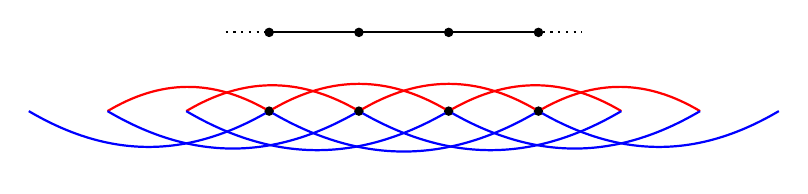
\begin{tikzpicture}[node distance=1.14cm,every node/.style=blacknode]
\node (0){} ;
\coordinate[left =0.5cm of 0] (a) ;
\node (1)[right of=0]{} ;
\node (2)[right of=1]{} ;
\node (3)[right of=2]{} ;
\coordinate[right =0.5cm of 3] (b) ;
\graph[edge={thick}]{(a)--[dotted](0)--(1)--(2)--(3)--[dotted](b)} ;

\begin{scope}[yshift=-1cm]
\node (0){} ;
%\coordinate[left =0.5cm of 0] (a) ;
\coordinate[left =1cm of 0] (-1) ;
\coordinate[left =2cm of 0] (-2) ;
\coordinate[left =3cm of 0] (-3) ;
\node (1)[right of=0]{} ;
\node (2)[right of=1]{} ;
\node (3)[right of=2]{} ;
%\node (4)[right of=3]{} ;
%\coordinate[right =0.5cm of 4] (b) ;
\coordinate[right =1cm of 3] (4) ;
\coordinate[right =2cm of 3] (5) ;
\coordinate[right =3cm of 3] (6) ;
\graph[edge={thick}]{(-2)--[bend left,red](0)--[bend left,red](2)--[bend left,red](4), (-1)--[bend left,red](1)--[bend left,red](3)--[bend left,red](5) } ;
\graph[edge={thick}]{(-3)--[bend right,blue](0)--[bend right,blue](3)--[bend right,blue](6), (-2)--[bend right,blue](1)--[bend right,blue](4),(-1)--[bend right,blue](2)--[bend right,blue](5)} ;
\end{scope}
\end{tikzpicture}
\caption{Fragments of two Cayley graphs of $\Z$ ($2$ ends), for the standard generating set $\{\pm1\}$ and for the generating set $\{\textcolor{red}{\pm2},\textcolor{blue}{\pm3}\}$.}
\label{Figure:CayleyOfZ}
\end{figure}
\begin{figure}[htbp]\centering
\begin{subfigure}{0.5\textwidth}
\centering
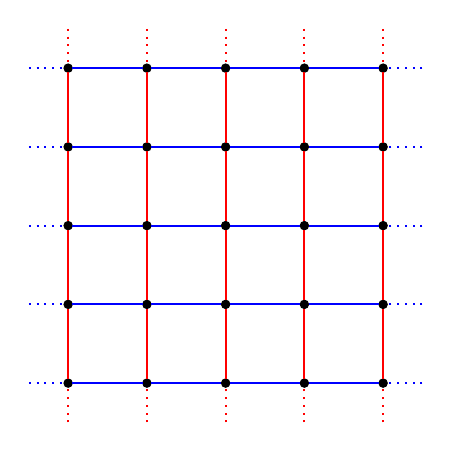
\begin{tikzpicture}
\foreach \i in {1,...,25}
{
        \pgfmathtruncatemacro{\y}{(\i - 1) / 5} ;
        \pgfmathtruncatemacro{\x}{\i - 5 * \y} ;
        \pgfmathtruncatemacro{\label}{\x + 5 * (4 - \y)} ;
        \node[blacknode] (\label) at (1*\x,-1*\y) {} ;
}
\foreach \i in {1,...,5}{
	\draw[thick, blue,dotted] (0.5,-\i+1)--(0.95,-\i+1) ;
	\draw[thick, blue,dotted] (5.5,-\i+1)--(5.05,-\i+1) ;
	\draw[thick, red,dotted] (\i,-4.5)--(\i,-4.05) ;
	\draw[thick, red,dotted] (\i,0.5)--(\i,0.05) ;
	\foreach \j in {0,...,3}{
		\pgfmathtruncatemacro{\x}{1+5*(\i-1)+\j} ;
		\pgfmathtruncatemacro{\y}{\x+1} ;
		\draw[thick, blue](\x)--(\y) ;
		\pgfmathtruncatemacro{\zz}{\i+5*\j} ;
		\pgfmathtruncatemacro{\t}{\zz+5} ;
		\draw[thick, red] (\zz)--(\t) ;
	}
}
\end{tikzpicture}
%\caption{Lorem ipsum}
\end{subfigure}%
\begin{subfigure}{0.5\textwidth}
\centering
\scalebox{0.8}{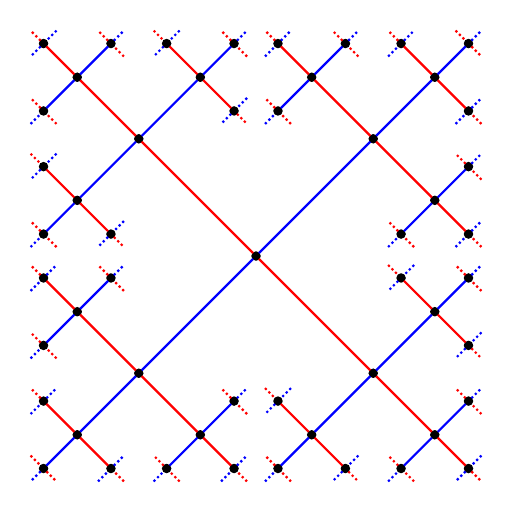
\begin{tikzpicture}[every node/.style=blacknode]
\useasboundingbox (-2.9,-2.9) rectangle (2.9,2.9);
\rotatebox{45}{
\node (0){};
\foreach \i/\j in {E/right,W/left}{
\node (\i)[\j = 2cm of 0]{} ;
\node (\i\i)[\j = 1cm of \i]{} ;
	\node (\i\i N)[above = 0.5cm of \i\i]{} ;
		\coordinate[above =0.18cm of \i\i N] (\i\i NN) ;
		\coordinate[right =0.18cm of \i\i N] (\i\i NE) ;
		\coordinate[left =0.18cm of \i\i N] (\i\i NW) ;
	\node (\i\i S)[below = 0.5cm of \i\i]{} ;
		\coordinate[below =0.18cm of \i\i S] (\i\i SS) ;
		\coordinate[right =0.18cm of \i\i S] (\i\i SE) ;
		\coordinate[left =0.18cm of \i\i S] (\i\i SW) ;
	\node (\i\i\i)[\j = 0.5cm of \i\i]{} ;
		\coordinate[\j =0.18cm of \i\i\i] (\i\i\i\i) ;
		\coordinate[above =0.18cm of \i\i\i] (\i\i\i N) ;
		\coordinate[below =0.18cm of \i\i\i] (\i\i\i S) ;
\node (\i N)[above = 1cm of \i ]{} ;
	\node (\i NN)[above = 0.5cm of \i N]{} ;
		\coordinate[above =0.18cm of \i NN] (\i NNN) ;
		\coordinate[right =0.18cm of \i NN] (\i NNE) ;
		\coordinate[left =0.18cm of \i NN] (\i NNW) ;
	\node (\i NW)[left = 0.5cm of \i N]{} ;
		\coordinate[above =0.18cm of \i NW] (\i NWN) ;
		\coordinate[below =0.18cm of \i NW] (\i NWS) ;
		\coordinate[left =0.18cm of \i NW] (\i NWW) ;
	\node (\i NE)[right = 0.5cm of \i N]{} ;
		\coordinate[above =0.18cm of \i NE] (\i NEN) ;
		\coordinate[below =0.18cm of \i NE] (\i NES) ;
		\coordinate[right =0.18cm of \i NE] (\i NEE) ;
\node (\i S)[below = 1cm of \i ]{} ;
	\node (\i SS)[below = 0.5cm of \i S]{} ;
		\coordinate[below =0.18cm of \i SS] (\i SSS) ;
		\coordinate[right =0.18cm of \i SS] (\i SSE) ;
		\coordinate[left =0.18cm of \i SS] (\i SSW) ;
	\node (\i SW)[left = 0.5cm of \i S]{} ;
		\coordinate[above =0.18cm of \i SW] (\i SWN) ;
		\coordinate[below =0.18cm of \i SW] (\i SWS) ;
		\coordinate[left =0.18cm of \i SW] (\i SWW) ;
	\node (\i SE)[right = 0.5cm of \i S]{} ;
		\coordinate[above =0.18cm of \i SE] (\i SEN) ;
		\coordinate[below =0.18cm of \i SE] (\i SES) ;
		\coordinate[right =0.18cm of \i SE] (\i SEE) ;
\graph[edge={thick,color=blue}]{
(0)--(\i )--(\i\i)--(\i\i\i)--[densely dotted](\i\i\i\i),
(\i SWW)--[densely dotted](\i SW)--(\i S)--(\i SE)--[densely dotted](\i SEE),
(\i NWW)--[densely dotted](\i NW)--(\i N)--(\i NE)--[densely dotted](\i NEE),
(\i NNW)--[densely dotted](\i NN)--[densely dotted](\i NNE),
(\i SSW)--[densely dotted](\i SS)--[densely dotted](\i SSE),
(\i\i NW)--[densely dotted](\i\i N)--[densely dotted](\i\i NE),
(\i\i SW)--[densely dotted](\i\i S)--[densely dotted](\i\i SE)
};
\graph[edge={thick,color=red}]{
	(\i SSS)--[densely dotted](\i SS)--(\i S)--(\i)--(\i N)--(\i NN)--[densely dotted](\i NNN),
	(\i\i SS)--[densely dotted](\i\i S)--(\i\i)--(\i\i N)--[densely dotted](\i\i NN),
	(\i\i\i N)--[densely dotted](\i\i\i)--[densely dotted](\i\i\i S),
	(\i NES)--[densely dotted](\i NE)--[densely dotted](\i NEN),
	(\i SES)--[densely dotted](\i SE)--[densely dotted](\i SEN),
	(\i NWS)--[densely dotted](\i NW)--[densely dotted](\i NWN),
	(\i SWS)--[densely dotted](\i SW)--[densely dotted](\i SWN)
};
}
\foreach \i/\j in {N/above,S/below}{
\node (\i)[\j = 2cm of 0]{} ;
\node (\i\i)[\j = 1cm of \i]{} ;
	\node (\i\i W)[left = 0.5cm of \i\i]{} ;
		\coordinate[above =0.18cm of \i\i W] (\i\i WN) ;
		\coordinate[below =0.18cm of \i\i W] (\i\i WS) ;
		\coordinate[left =0.18cm of \i\i W] (\i\i WW) ;	
	\node (\i\i E)[right = 0.5cm of \i\i]{} ;
		\coordinate[above =0.18cm of \i\i E] (\i\i EN) ;
		\coordinate[below =0.18cm of \i\i E] (\i\i ES) ;
		\coordinate[right =0.18cm of \i\i E] (\i\i EE) ;
	\node (\i\i\i)[\j = 0.5cm of \i\i]{} ;
		\coordinate[\j =0.18cm of \i\i\i] (\i\i\i\i) ;
		\coordinate[right =0.18cm of \i\i\i] (\i\i\i E) ;
		\coordinate[left =0.18cm of \i\i\i] (\i\i\i W) ;
\node (\i E)[right = 1cm of \i ]{} ;
	\node (\i EE)[right = 0.5cm of \i E]{} ;
		\coordinate[above =0.18cm of \i EE] (\i EEN) ;
		\coordinate[below =0.18cm of \i EE] (\i EES) ;
		\coordinate[right =0.18cm of \i EE] (\i EEE) ;
	\node (\i ES)[below = 0.5cm of \i E]{} ;
		\coordinate[below =0.18cm of \i ES] (\i ESS) ;
		\coordinate[left =0.18cm of \i ES] (\i ESE) ;
		\coordinate[right =0.18cm of \i ES] (\i ESW) ;
	\node (\i EN)[above = 0.5cm of \i E]{} ;
		\coordinate[above =0.18cm of \i EN] (\i ENN) ;
		\coordinate[left =0.18cm of \i EN] (\i ENE) ;
		\coordinate[right =0.18cm of \i EN] (\i ENW) ;
\node (\i W)[left = 1cm of \i ]{} ;
	\node (\i WS)[below = 0.5cm of \i W]{} ;
		\coordinate[below =0.18cm of \i WS] (\i WSS) ;
		\coordinate[left =0.18cm of \i WS] (\i WSE) ;
		\coordinate[right =0.18cm of \i WS] (\i WSW) ;
	\node (\i WN)[above = 0.5cm of \i W]{} ;
		\coordinate[above =0.18cm of \i WN] (\i WNN) ;
		\coordinate[left =0.18cm of \i WN] (\i WNE) ;
		\coordinate[right =0.18cm of \i WN] (\i WNW) ;
	\node (\i WW)[left = 0.5cm of \i W]{} ;
		\coordinate[above =0.18cm of \i WW] (\i WWN) ;
		\coordinate[below =0.18cm of \i WW] (\i WWS) ;
		\coordinate[left =0.18cm of \i WW] (\i WWW) ;
\graph[edge={thick,color=red}]{
	(0)--(\i )--(\i\i)--(\i\i\i)--[densely dotted](\i\i\i\i),
	(\i ENN)--[densely dotted](\i EN)--(\i E)--(\i ES)--[densely dotted](\i ESS),
	(\i WNN)--[densely dotted](\i WN)--(\i W)--(\i WS)--[densely dotted](\i WSS),
	(\i EES)--[densely dotted](\i EE)--[densely dotted](\i EEN),
	(\i WWS)--[densely dotted](\i WW)--[densely dotted](\i WWN),
	(\i\i ES)--[densely dotted](\i\i E)--[densely dotted](\i\i EN),
	(\i\i WS)--[densely dotted](\i\i W)--[densely dotted](\i\i WN)};
\graph[edge={thick,color=blue}]{
	(\i WWW)--[densely dotted](\i WW)--(\i W)--(\i)--(\i E)--(\i EE)--[densely dotted](\i EEE),
	(\i\i WW)--[densely dotted](\i\i W)--(\i\i)--(\i\i E)--[densely dotted](\i\i EE),
	(\i ENW)--[densely dotted](\i EN)--[densely dotted](\i ENE),
	(\i ESW)--[densely dotted](\i ES)--[densely dotted](\i ESE),
	(\i WNW)--[densely dotted](\i WN)--[densely dotted](\i WNE),
	(\i WSW)--[densely dotted](\i WS)--[densely dotted](\i WSE),
	(\i\i\i E)--[densely dotted](\i\i\i)--[densely dotted](\i\i\i W)};
}
}
\end{tikzpicture}}
%\caption{Lorem ipsum}
\end{subfigure}
\caption{Fragments of the Cayley graphs of $\Z^2$ ($1$ end) on the left and of $F_2$ (infinitely many ends) on the right; with standard generating sets.}
\label{Figure:CayleyOfZ2}
\end{figure}
\begin{figure}[htbp]\centering
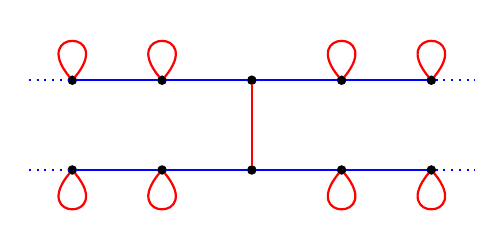
\begin{tikzpicture}[node distance=1.14cm,every node/.style=blacknode]
\node (00){} ;
\coordinate[left =0.5cm of 00] (0a) ;
\node (01)[right of=00]{} ;
\node (02)[right of=01]{} ;
\node (03)[right of=02]{} ;
\node (04)[right of=03]{} ;
\coordinate[right =0.5cm of 04] (0b) ;
\node (10)[above of=00]{} ;
\coordinate[left =0.5cm of 10] (1a) ;
\node (11)[above of=01]{} ;
\node (12)[above of=02]{} ;
\node (13)[above of=03]{} ;
\node (14)[above of=04]{} ;
\coordinate[right =0.5cm of 14] (1b) ;
\graph[edge={thick,color=blue}]{(0a)--[dotted](00)--(01)--(02)--(03)--(04)--[dotted](0b)} ;
\graph[edge={thick,color=blue}]{(1a)--[dotted](10)--(11)--(12)--(13)--(14)--[dotted](1b)} ;
\graph[edge={thick,color=red}]{(02)--(12)} ;
\foreach \i in {0,1,3,4}{
\draw [thick,color=red] (0\i) to [myloop below] (0\i) ;
\draw [thick,color=red] (1\i) to [myloop above] (1\i) ;
}
%\begin{scope}[yshift=-1cm]
%\node (0){} ;
%%\coordinate[left =0.5cm of 0] (a) ;
%\coordinate[left =1cm of 0] (-1) ;
%\coordinate[left =2cm of 0] (-2) ;
%\coordinate[left =3cm of 0] (-3) ;
%\node (1)[right of=0]{} ;
%\node (2)[right of=1]{} ;
%\node (3)[right of=2]{} ;
%%\node (4)[right of=3]{} ;
%%\coordinate[right =0.5cm of 4] (b) ;
%\coordinate[right =1cm of 3] (4) ;
%\coordinate[right =2cm of 3] (5) ;
%\coordinate[right =3cm of 3] (6) ;
%\graph[edge={thick}]{(-2)--[bend left,red](0)--[bend left,red](2)--[bend left,red](4), (-1)--[bend left,red](1)--[bend left,red](3)--[bend left,red](5) } ;
%\graph[edge={thick}]{(-3)--[bend right,blue](0)--[bend right,blue](3)--[bend right,blue](6), (-2)--[bend right,blue](1)--[bend right,blue](4),(-1)--[bend right,blue](2)--[bend right,blue](5)} ;
%\end{scope}
\end{tikzpicture}
\caption{A fragment of a Schreier graph (with $4$ ends) of the free group $F_2=\langle \textcolor{red}{x^{\pm1}},\textcolor{blue}{y^{\pm1}}\rangle$.}
\label{Figure:SchreierOfF2}
\end{figure}
%
%
Let $\Gamma$ be a graph and $K$ a finite subset of vertices. The graph $\Gamma\setminus K$ is the subgraph of $\Gamma$ obtained by deleting all vertices in $K$ and all edges adjacent to them. This graph is not necessarily connected.
\begin{defn}\label{Def:Ends}
Let $\Gamma$ be a graph. The \emph{number of ends} of $\Gamma$ is the supremum, taken over all finite $K$, of the number of infinite connected components of $\Gamma\setminus K$.
\end{defn}
There exists other characterization of the number of ends in graphs, %notably in terms of equivalence classes of rays,
see \cite{MR1967888} and the references therein, but Definition \ref{Def:Ends} is the one that best suits our purpose.
%The interested reader may refer to \cite{MR1967888} and the references therein for an extended treatment of the 
A locally finite graph (i.e. such that every vertex has finite degree) is finite if and only if it has $0$ ends.
%The graphs of the Figures~\ref{Figure:CayleyOfZ} and \ref{Figure:CayleyOfZ2} have respectively 2 ends and 1 end. 

An important fact about the number of ends of a graph, is that it is an invariant of quasi-isometry, see \cite{MR1213151}. In particular, if $G$ is a finitely generated group it is possible to speak about the number of ends of the Schreier graph $\Sch(G,H;S)$ without specifying a particular finite generating set $S$.
By a celebrated result of Stallings \cite{Stallings1971}, the number of ends of a Cayley graph of a finitely generated group can only be $0$, $1$, $2$ or infinite (in which case it is uncountable), see Figures~\ref{Figure:CayleyOfZ} and \ref{Figure:CayleyOfZ2} for examples.
On the other hand, Schreier graphs may have any number of ends in $\mathbf N\cup\{\infty\}$, see Figure~\ref{Figure:SchreierOfF2} for an example of a graph with $4$ ends.
%While the number of ends of Cayley graphs of finitely generated groups can only be $0$, $1$, $2$ or infinite (in which case it is uncountable) \cite[Theorem 11.27]{Stallings1971}, Schreier graphs may have any number of ends in $\mathbf N\cup\{\infty\}$, see Figure~\ref{Figure:SchreierOfF2} for an example of a graph with another number of ends.
In fact, every regular graph of even degree is isomorphic to a Schreier graph, \cite{MR0450121,MR1358635}. 

We are now finally able to introduce property FW. The following characterization is due to Cornulier \cite{Cornulier2013}.
%
%
\begin{defn}
A finitely generated group $G$ has \emph{property FW} if all its Schreier graphs have at most one end.
\end{defn}
%
%
It directly follows from the definition that all finite groups have property FW, but that $\Z$ does not have it.
In fact, if $G$ is a finitely generated group with an homomorphism onto $\Z$, then it does not have FW. Indeed, in this case $G\cong H\rtimes \Z$  for some $H$ and the Schreier graph $\Sch(G,H;S)$ will be isomorphic to a Cayley graph of $\Z\cong G/H$ and hence has $2$ ends.

Property FW admits many distinct characterizations that allow to define it for groups that are non-necessarily finitely generated and even for topological groups. We refer the reader to \cite{Cornulier2013} for a survey of these characterizations.
%
%
%
%
%
%
%
%
%
%
%%%%%%%%%%%%%%%%%%%%%%%%%%%%%%%%%%%%%%%%%%%%%%%%%%%%%%%%%%%%%%%%%%%%%%%%%%%
%%%%%%%%%%%%%%%%%%%%%%%%%%%%%%%%%%%%%%%%%%%%%%%%%%%%%%%%%%%%%%%%%%%%%%%%%%%
%%%%%%%%%%%%%%%%%%%%    Subsection : Wreath products    %%%%%%%%%%%%%%%%%%%
%%%%%%%%%%%%%%%%%%%%%%%%%%%%%%%%%%%%%%%%%%%%%%%%%%%%%%%%%%%%%%%%%%%%%%%%%%%
%%%%%%%%%%%%%%%%%%%%%%%%%%%%%%%%%%%%%%%%%%%%%%%%%%%%%%%%%%%%%%%%%%%%%%%%%%%
\subsection{Wreath products}
%
%
%
%
%
Let $X$ be a set and $G$ a group. We view 
$\bigoplus_XG$ as the set of functions from $X$ to $G$ with finite support:
\[
	\bigoplus_XG=\setst{\varphi\colon X\to G}{\varphi(x)=1 \textnormal{ for all but finitely many }x}.
\]
This is naturally a group, where multiplication is taken componentwise.

If $H$ is a group acting on $X$, then it naturally acts on $\bigoplus_XG$
by $(h.\varphi)(x)=\varphi(h^{-1}.x)$.
This leads to the following definition
\begin{defn}\label{Def:WreathProd}
Let $G$ and $H$ be groups and $X$ be a set on which $H$ acts.
The \emph{(retricted) wreath product} $G\wr_XH$ is the group $(\bigoplus_XG)\rtimes H$.
\end{defn}
A prominent  source of examples of wreath products are the ones of the form $G\wr_HH$, where $H$ acts on itself by left multiplication.
In particular, the group $(\Z/2\Z)\wr_\Z\Z$ has become well-known under the name of the \emph{lamplighter group}.
Another (trivial) examples of wreath products are direct products $G\times H$ which corresponds to wreath products over a singleton $G\wr_{\{*\}}H$.

Let $S$ be a generating set of $G$ and $T$ a generating set of $H$.
Suppose that $H$ acts transitively on $X$ and let $x\in X$ be any point.
Finally, let $\delta_x^s$ be the element of $\bigoplus_XG$ defined by $\delta_x^s(x)=s$ and $\delta_x^s(y)=1_G$ if $y\neq x$ and let $\mathbf 1$ be the constant function with value $1$.
It is then standard that 
\[
	\setst{(\delta_x^s,1_H)}{s \in S} \cup \setst{(\mathbf 1,t}{t \in T}
\]
is a generating set for $G\wr_XH$.

On the other hand, it follows from the definition of the wreath product that we have
\[
	G\wr_XH\cong\bigoplus_{Y\textnormal{ is an $H$-orbit}}\bigl(G\wr_YH\bigr).
\]
We hence obtain
%
%
\begin{lem}
The group $G\wr_XH$ is finitely generated if and only if both $G$ and $H$ are finitely generated and $H$ acts on $X$ with finitely many orbits.
\end{lem}
%
%
Using the above lemma, we could reformulate Theorem~\ref{Thm:Main} in the following way:
%
%
\begin{prop}
Let $G$, $H$ be two groups with $G$ non-trivial and $X$ a set on which $H$ acts. Suppose that all three of $G$, $H$ and $G\wr_XH$ are finitely generated. Then the wreath product $G\wr_XH$ has property FW if and only if $G$ and $H$ have property FW and $X$ is finite.
\end{prop}
%!TEX root = ends.tex
%
%
%
%
%
%
%
%
%
%
%%%%%%%%%%%%%%%%%%%%%%%%%%%%%%%%%%%%%%%%%%%%%%%%%%%%%%%%%%%%%%%%%%%%%%%%%%%
%%%%%%%%%%%%%%%%%%%%%%%%%%%%%%%%%%%%%%%%%%%%%%%%%%%%%%%%%%%%%%%%%%%%%%%%%%%
%%%%%%%%%%%%%%%%%    Section : Proof of the main result    %%%%%%%%%%%%%%%%
%%%%%%%%%%%%%%%%%%%%%%%%%%%%%%%%%%%%%%%%%%%%%%%%%%%%%%%%%%%%%%%%%%%%%%%%%%%
%%%%%%%%%%%%%%%%%%%%%%%%%%%%%%%%%%%%%%%%%%%%%%%%%%%%%%%%%%%%%%%%%%%%%%%%%%%
\section{Proof of the main result}
\label{Section:Proof}
%
%
%
%
%
This section is devoted to the proof of Theorem~\ref{Thm:Main}. This proof is split into two parts: Lemma \ref{Lemma:Semidirect_ends} and its Corollary \ref{Cor:Wreath_ends} and Lemma \ref{Lem:Wreath_groups_ends}.
We then conclude by a result on finite index subgroups.

\todo[inline]{Est-ce qu'on veut rajouter que si $H$ est un sous-groupe d'indice fini de $G$, alors $G$ a FW ssi $H$ a FW ? C'est le seul petit résultat qui fait sens à prouver. En effet, ceux sur les sommes directes font intervenir des groupes qui ne sont pas de type fini.}

We begin by a result on semi-direct products.
%
%
\begin{lem}\label{Lemma:Semidirect_ends}
Let $N$ and $H$ be two finitely generated groups and $N\rtimes H$ a semi-direct product.
Then
\begin{enumerate}
\item If $N\rtimes H$ has FW, then so does $H$,
\item If both $N$ and $H$ have FW, then $G$ also has FW.
\end{enumerate}
\end{lem}
%
%
\begin{proof}
Let $S$, respectively $T$, denotes a finite generating set of $N$, respectively $H$.
It is well known that $G=N\rtimes H$ is finitely generated by $U=(S\times\{1\}) \cup(\{1\}\times T)$.

Suppose that $H$ does not have property FW. Then there exists a Schreier graph $\Gamma=\Sch(H,K;T)$ of $H$ with more than one end. The group $G=N\rtimes H$ acts on $\Gamma$ via $(n,h).x \coloneqq h.x$.
Since $H$ acts transitively on $\Gamma$, so does $G$.
In fact, the graph of the action $G$ on the vertices of $\Gamma$ is isomorphic to the graph $\Gamma$ with some additional loops for generators in $S\times\{1\}$. As adding loops does not change the number of ends, this Schreier graph has more than one end and therefore $G$ does not have property FW.

Suppose now that both $N$ and $H$ have property FW. We want to show that every Schreier graphs of $G$ have at most one end. If they are all finite, then there is nothing to prove (and $G$ is finite). So let $\Gamma$ be an infinite Schreier graph of $G$ with respect to the generating set $U$. The groups $N$ and $H$ acts on $\Gamma$ by restriction of the action of $G$. That is, $n.x = (n,1).x$ and $h.x = (1,h).x$ for $x$ a vertex of $\Gamma$.
For each vertex $x$ we define $\Gamma_x^H$ (and respectively $\Gamma_x^N$) as the Schreier graph obtained from the action of $H$ (respectively $N$) on the $H$-orbit (respectively $N$-orbit) of $x$. These are subgraphs of $\Gamma$. As $N$ and $H$ have property FW, the graphs $\Gamma_x^H$ and $\Gamma_x^N$ are either finite or one-ended. We want to prove that in this case $\Gamma$ has exactly one end. 

Let $K$ be a finite set of vertices of $\Gamma$.
If $x$ is in $K$ and $\Gamma_x^H$ is finite, add all vertices of $\Gamma_x^H$ to $K$.
By doing so for every $x$ in $K$, we obtain a new finite set $K\subset K'$ of vertices of $\Gamma$.
We will show that $\Gamma\setminus K'$ has only one infinite connected component.
By definition of $K'$, if $x$ is not in $K'$, then either $\Gamma_x^H$ has one end or $\Gamma_x^H$ does not contains vertices in $K'$. 

Let $x$ and $y$ be two vertices, each of them lying in some infinite connected component of $\Gamma\setminus K'$.
We will construct a path from $x$ to $y$ in $\Gamma\setminus K'$ as a concatenation of three smaller paths as follow, see Figure~\ref{Figure:PathSemiDirect}.
First, a path in $\Gamma_x^H\setminus K'$ from $x$ to some $z$, then a path in $\Gamma_z^N\setminus K'$ from $z$ to some $z'\in (\Gamma_z^N\cap \Gamma_y^H)\setminus K'$, and finally a path in $\Gamma_y^H\setminus K'$ from $z'$ to $y$.
In order to finish the proof, it remains to exhibit elements $z$ and $z'$ and the three desired paths.
%
%
\begin{figure}[htbp]\centering
\scalebox{0.7}{
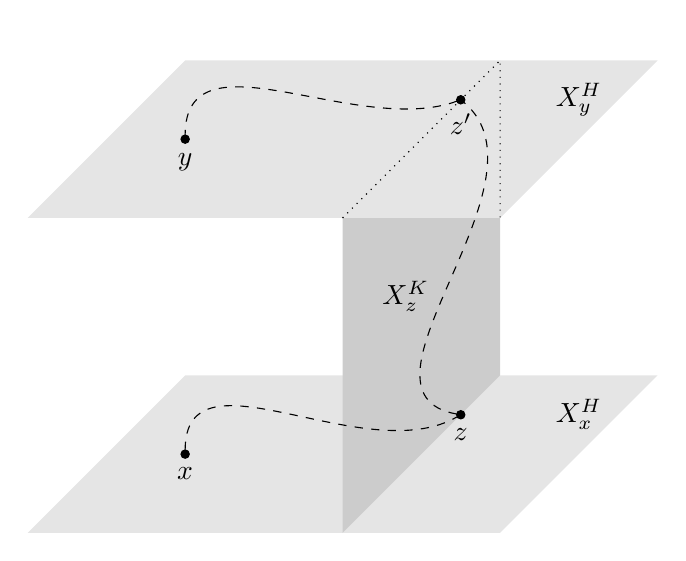
\begin{tikzpicture}
\fill[color = gray!20] (-4,0) -- (2,0) --(4,2) -- (-2,2) --cycle;
\fill[color = gray!40] (0,0) -- (2,2) --(2,6) -- (0,4) --cycle;
\fill[color = gray!20] (-4,4) -- (2,4) --(4,6) -- (-2,6) --cycle;
\draw [dotted] (0,4) -- (2,6) --(2,4);
\draw (3,1.5) node {$X_x^H$};
\draw (0.8,3) node {$X_z^K$};
\draw (3,5.5) node {$X_y^H$};
\node[style=blacknode, label={below:$x$}] (x) at (-2,1) {};
\node[style=blacknode, label={below:$z$}]  (z) at (1.5,1.5) {};
\node[style=blacknode, label={below:$z'$}]  (z') at (1.5,5.5) {};
\node[style=blacknode, label={below:$y$}]  (y) at (-2,5) {};
\draw [dashed] (x) to [out=90,in=210] (z) to [out=170,in=-40] (z') to [out=200,in=90] (y) ;
\end{tikzpicture}}
\caption{The path between $x$ and $y$.}
\label{Figure:PathSemiDirect}
\end{figure}
%
%

The action of $G$ on $\Gamma$ being transitive, there exists an element $(n_0,h_0)$ of $N \rtimes H$ such that $(n_0,h_0).x = y$.
Since $K'$ is finite, the set $\Gamma_x^H\setminus K'$ is infinite.
Moreover, there is infinitely many $z$ in $\Gamma_x^H\setminus K'$ such that either $\Gamma_z^N$ is one-ended or $\Gamma_z^N$ does not intersect $K'$.
For such a $z$ there exists $h$ such that $(1,h).x=z$.
Now, the vertex $z'\coloneqq(hh_0^{-1}n_0,h).x$ is both equal to $(hh_0^{-1}.n_0,1)(1,h_0).x=(hh_0^{-1}.n_0,1).z$ and to $(1,hh_0^{-1})(n_0,h_0).x=(1,hh_0^{-1}).y$. That is, $z'$ is in $\Gamma_z^N\cap X_y^H$.
A simple computation show us that the map $z\mapsto z'$ is injective: $z_1'=z_2'$ if and only if $z_1=z_2$.
Since $K'$ is finite, there is only finitely many $z'$ in $K'$ and hence there is infinitely many $z\in \Gamma_x^H$ such that both $z$ and $z'$ are not in $K'$ and either $\Gamma_z^N$ is one-ended or $\Gamma_z^N$ does not intersect $K'$.

In order to finish the proof, observe that the three graphs $\Gamma_x^H$, $\Gamma_y^H$ and $\Gamma_z^N$ are all either one-ended or do not intersect $K'$.
Therefore, there is a path in $\Gamma_x^H\setminus K'$ from $x$ to $z$ as desired, and so on for the paths from $z$ to $z'$ and $z'$ to $y$.
We just have proved that for any finite $K$ the graph $\Gamma\setminus K$ has only one infinite connected component and therefore that $\Gamma$ is one-ended.
\end{proof}
%
%
By iterating the last lemma, we obtain
%
%
\begin{cor}\label{Cor:Wreath_ends}
Let $G$ and $H$ be two finitely generated groups and $X$ a $H$-set such that the number of orbits is finite. Then,
\begin{enumerate}
\item
If $G\wr_X H$ has property FW, then so does $H$,
\item
If both $G$ and $H$ have property FW and $X$ is finite, then $G\wr_X H$ has property~FW.
\end{enumerate}
\end{cor}
%
%
The following Lemma finishes the proof of Theorem~\ref{Thm:Main}.
%
%
\begin{lem}\label{Lem:Wreath_groups_ends}
Let $G$ and $H$ be two finitely generated groups such that $G\neq \{1\}$ and $H$ acts on some set $X$ with finitely many orbits.
If $G\wr_XH$ has property FW, then 
\begin{enumerate}
\item $G$ has property FW,
\item $X$ is finite.
\end{enumerate}
\end{lem}
%
%
\begin{proof}
We will prove the contrapositives. The idea is to construct, for each of the two cases, a Schreier graph of $G\wr_XH$ with more than one end by exhibiting some well-chosen action of $G\wr_XH$.
We fix some finite generating sets $S$ and $T$ of $G$ and $H$ and let 
\[
	U\coloneqq\setst{(\delta_x^s,1_H)}{s \in S} \cup \setst{(\mathbf 1,t}{t \in T}
\]
be the standard generating set of $G\wr_XH$.
%
%
%
\paragraph{Suppose that $X$ is an infinite set.}
Since $H$ acts on $X$ with finitely many orbits, there exists an infinite orbit $X'$.
Let $x_0$ be an arbitrary vertex of $X'$.
The group $G$ acting on itself by left multiplications, we have the so-called \emph{imprimitive action} of the wreath-product $G\wr_XH$ on $Y\coloneqq G\times X'$:
\[
	(\varphi,h). (g,x) \coloneqq (\varphi(h.x)g, h.x).
\]
Since both $G\curvearrowright G$ and $H\curvearrowright X'$ are transitive, the action $G\wr_XH\curvearrowright Y$ is also transitive. 
Therefore, the orbital Schreier graph of $G\wr_XH\curvearrowright Y$ is isomorphic to the Schreier graph $\Gamma\coloneqq\Sch(G\wr_XH, \stab(1_G,x_0), U)$. We decompose this graph into leaves of the form $Y_g = \{ g \} \times X'$. There are two types of edges in $\Gamma$, which are coming from the two sets of generators, see Figure~\ref{Figure:Leaves}. The first ones, of the form $(\mathbf 1,t)$, give us on each leaf a copy of the orbital Schreier graph of $H \curvearrowright X'$. Indeed,
\[
	(\mathbf 1,t).(g,x) = (g, t.x).
\]
The second ones, of the form $(\delta_{x_0}^s,1)$, give us loops everywhere except on vertices of the form $(g,x_0)$. By direct computation, we see that the vertices $(g,x_0)$ and $(sg,x_0)$ connect the leaves $Y_g$ and $Y_{sg}$, 
\[
	(\delta_{x_0}^s,1).(g,x) = 
		\begin{cases}
		(g,x) & \textnormal{if }x \neq x_0, \\
		(sg, x) & \textnormal{if }x = x_0.
		\end{cases}
\]
%
%
\begin{figure}[htbp]\centering
\scalebox{0.7}{
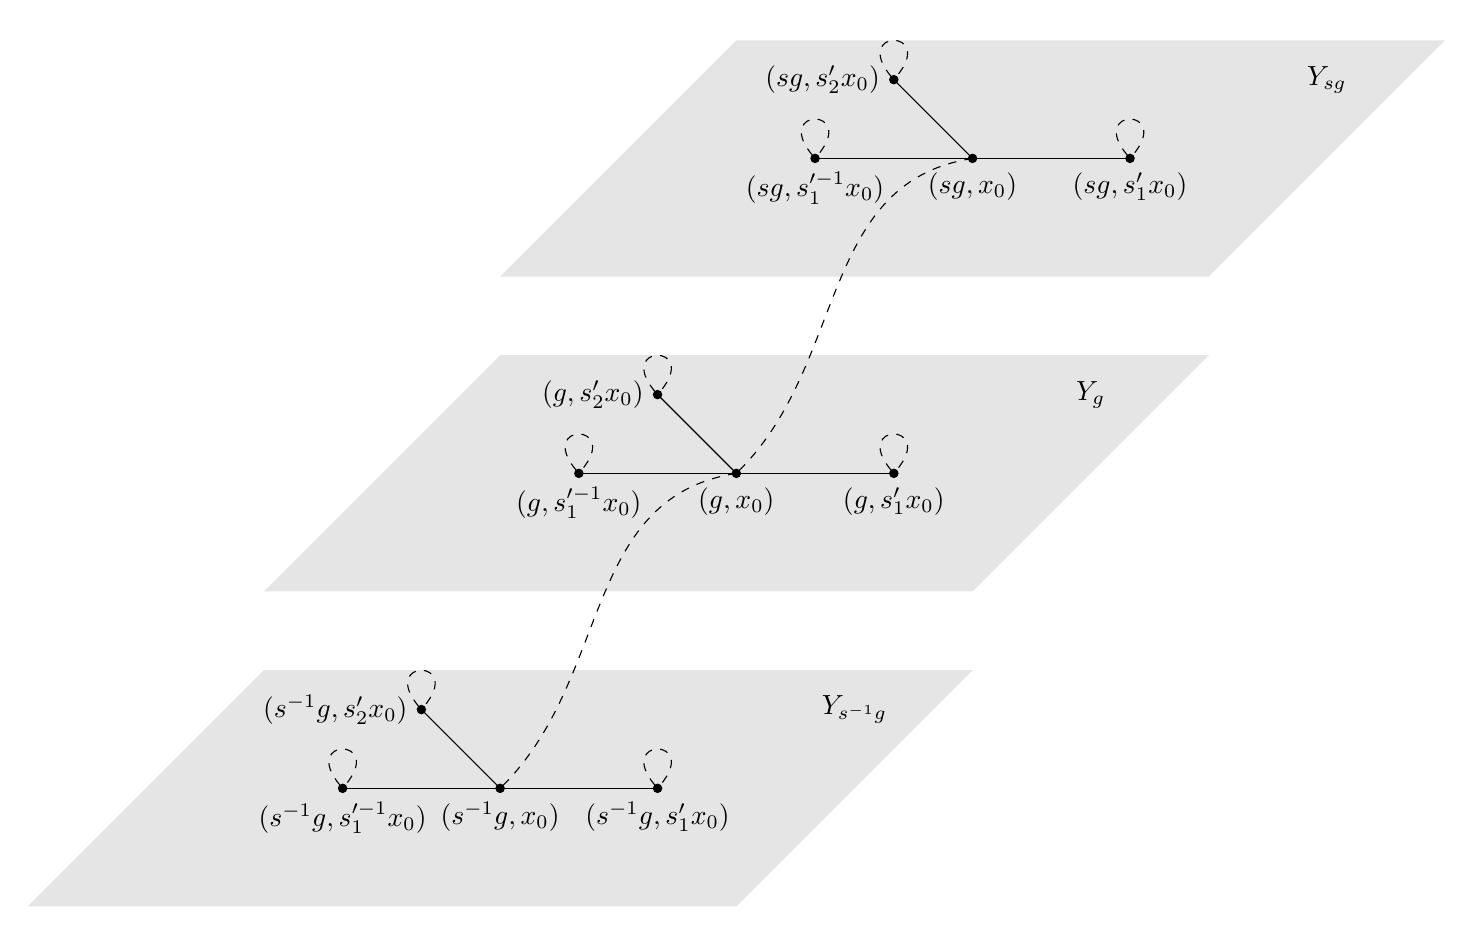
\begin{tikzpicture}
\fill[color = gray!20] (-6,-1.5) -- (3,-1.5) --(6,1.5) -- (-3,1.5) --cycle;
\draw (4.5,1) node {$Y_g$};
\node[style=blacknode, label= {below:$(g,x_0)$}] (00) at (0,0) {};
\node[style=blacknode, label={below:$(g,s'_1x_0)$}] (10) at (2,0) {};
\node[style=blacknode, label={below:$(g,s'^{-1}_1x_0)$}] (-10) at (-2,0) {};
\node[style=blacknode, label={left:$(g,s'_2x_0)$}] (20) at (-1,1) {};
\draw(-10) -- (00) -- (10);
\draw (20) -- (00);

\begin{scope}[shift = {(3,4)}]
\fill[color = gray!20] (-6,-1.5) -- (3,-1.5) --(6,1.5) -- (-3,1.5) --cycle;
\draw (4.5,1) node {$Y_{sg}$};
\node[style=blacknode, label={below:$(sg,x_0)$}] (01) at (0,0) {};
\node[style=blacknode, label={below:$(sg,s'_1x_0)$}] (11) at (2,0) {};
\node[style=blacknode, label={below:$(sg,s'^{-1}_1x_0)$}] (-11) at (-2,0) {};
\node[style=blacknode, label={left:$(sg,s'_2x_0)$}] (21) at (-1,1) {};
\draw(-11) -- (01) -- (11);
\draw (21) -- (01);
\end{scope}

\begin{scope}[shift = {(-3,-4)}]
\fill[color = gray!20] (-6,-1.5) -- (3,-1.5) --(6,1.5) -- (-3,1.5) --cycle;
\draw (4.5,1) node {$Y_{s^{-1}g}$};
\node[style=blacknode, label={below:$(s^{-1}g,x_0)$}] (02) at (0,0) {};
\node[style=blacknode, label={below:$(s^{-1}g,s'_1x_0)$}] (12) at (2,0) {};
\node[style=blacknode, label={below:$(s^{-1}g,s'^{-1}_1x_0)$}] (-12) at (-2,0) {};
\node[style=blacknode, label={left:$(s^{-1}g,s'_2x_0)$}] (22) at (-1,1) {};
\draw(-12) -- (02) -- (12);
\draw (22) -- (02);\end{scope}
\draw [dashed] (02) to [out=45,in=190] (00) to [out=45,in=190] (01);
\draw [dashed] (10) to [myloop above] (10) ;
\draw [dashed] (20) to [myloop above] (20) ;
\draw [dashed] (-10) to [myloop above] (-10) ;
\draw [dashed] (11) to [myloop above] (11) ;
\draw [dashed] (21) to [myloop above] (21) ;
\draw [dashed] (-11) to [myloop above] (-11) ;
\draw [dashed] (12) to [myloop above] (12) ;
\draw [dashed] (22) to [myloop above] (22) ;
\draw [dashed] (-12) to [myloop above] (-12) ;
\end{tikzpicture}}
\caption{The leaf structure of the orbital Schreier graph of $G\wr_XH \curvearrowright Y$. Plain edges correspond to generators of the form $(\mathbf 1,t)$ while dotted edges correspond to generators of the form $(\delta_{x_0}^s,1)$.}
\label{Figure:Leaves}
\end{figure}
%
%

If we remove a vertex $(g,x_0)$ we disconnect the leaf $Y_g$ from the rest of $\Gamma$. As $X'$ is infinite each leave is infinite and the number of ends of $\Gamma$ is then at least $\abs{G}\geq 2$. We just proved that if $X$ is infinite the group $G\wr_XH$ does not have property FW.
%
%
%
\paragraph{Suppose now that $G$ does not have property FW.} There exists a subgroup $K$ of $G$ such that $\Sch(G,K,S)$ has more than one end.
Let $x_0$ be any point of $X$ and $X'$ be its orbit under the action of $H$.
We have the imprimitive action of $G\wr_XH$ on $G/K\times X$, which we could restrict to an action on $G/K\times X'$:
\[
	(\varphi,h).(gK,x) = (\varphi(h.x) gK, h.x).
\]
As above, the action is transitive and the orbital Schreier graph of this action is isomorphic to a Schreier graph $\Gamma$. We decompose this graph into leaves in the same way. Now we look at the subgraph made up of vertices $(g,x_0)$ and edges $(\delta_{x_0}^s,1)$ and we remark that it is isomorphic to the Schreier graph $\Sch(G,K,S)$ which has more than one end. Then $\Gamma$ has also more than one end, which finishes the proof.
\end{proof}
%
%
We conclude this note by recording the following result on finite index subgroups.
%
%
\begin{lem}
Let $G$ be a finitely generated subgroup and let $H\leq G$ be a finite index subgroup. Then $G$ has property FW if and only if $H$ has property FW.
\end{lem}
%
%
\begin{proof}
Since $H$ is a finite index subgroup of the finitely generated group $H$, it is itself finitely generated.
So let $S$ be a finite symmetric generating set for $H$ and let $\{g_1,\dots, g_n\}$ be a set of representatives of $G/H$.
Then $T=S\cup\{g_1^\pm,\dots, g_n^\pm\}$ is a finite symmetric generating set for $G$.

Suppose that $H$ has property FW and let $\Gamma$ be a Schreier graph of $G$ with respect to $T$.
\end{proof}
%
%
%
%
%
%
%
%
%
%
\bibliography{biblio.bib}
\bibliographystyle{plain}
%
%
%
%
%
\enddocument